\documentclass[../main/main.tex]{subfiles}

\begin{document}

\section{February 8th, 2022}
\subsection{Fundamental Principles of Statistical Mechanics}
Statistical mechanics is the basis for computer simulation at molecular scale. For this we can simulate the behavior of each molecule/atom (\vocab{microscopic}), but we can also study
the collective behavior of large number of molecules/atoms (\vocab{macroscopic}). Statistical mechanics provides a link from microscopic scale to macroscopic.

\subsection{Review of Classical Mechanics}

\subsubsection{The Lagrangian}
Consider a system described by:
\begin{itemize}
	\item Generalized coordinates $q_i$
	\item Velocity $\dot{q_i}\left( \frac{dq_i}{dt} \right)$.
\end{itemize}

The \vocab{Lagrangian} is: \[
	L = L(\q, \dot{\q}) = \sum\limits_{i=1}^{s} \frac{1}{2} m_i \dot{q}_i^2 - U(\q)
\]
where:
\begin{itemize}
	\item $s$: degrees of freedom
	\item $m_i$: mass associated with $q_i$
	\item $U$: potential energy depending only on $\q = (q_1, q_2, \ldots,q_s)$
	\item $\sum\limits_{i=1}^{s} \frac{1}{2} m_i \dot{q}_i^2$: kinetic energy
\end{itemize}

\begin{remark}
	Since we can use a generalized coordinate system, this will be useful for dealing with other coordinate systems, such as polar.
\end{remark}

Action is defined as: \[
	S = \int\limits_{t_1}^{t_2}L(\q,\dot{\q})
\]
Fix $\q(t_1) = \q^{(1)}, \q(t_2) = \q^{(2)}$. There are infinitely many paths that connect $\q^{(1)}$ and $\q^{(2)}$. The \vocab{principle of least action}
says that the path taken is the one with least action.\\

When $S(\q)$a is the least value, we have: \[
	S(\q + \delta \q) = \int\limits_{t_1}^{t_2}L(\q+\delta \q, \dot{\q}+ \delta \dot{\q}) dt \geq S(\q)
\]
We have:
\begin{align*}
	S(\q+ \delta \q) -S(\q) & = \int\limits_{t_1}^{t_2} [L(\q+ \delta \q , \dot{\q} + \delta \dot{\q}) - L(\q,\dot{\q})] dt                                                                                                     \\
	                        & \approx  \int\limits_{t_1}^{t_2} \left[ \sum\limits_{i=1}^{s} \frac{\partial L}{\partial q_1}  \delta q_i + \sum\limits_{i=1}^{s} \frac{\partial L}{\partial \dot{q}} \delta \dot{q_i} \right] dt \\
	                        & = \int\limits_{t_1}^{t_2} \sum\limits_{i=1}^{s} \left[ \frac{\partial L}{\partial q_i } - \frac{d}{dt} \frac{\partial L}{\partial \dot{q}} \right].
\end{align*}

This holds for any $\delta q_i$, thus: \[
	\frac{\partial L}{\partial q_i} - \frac{d}{dt} \frac{\partial L}{\partial \dot{q}} = 0, \quad i = 1,2, \ldots, s
\]
This is the \textbf{Lagrangian formulation} of classical mechanics.
This is an alternative expression of Newton's equations. In addition, this formulation is convenient for generalized coordinates.

\begin{example}
	Let us consider the example where we have a particle moving under a one-dimensional potential $U(x)$, where $x$ is the location. We have: \[
		L(x, \dot{x}) = \frac{1}{2} m \dot{x}^2 - U(x)
	\] Thus the action is: \[
		S = \int\limits_{t_1}^{t_2}L(x, \dot{x}) dt = \int\limits_{t_1}^{t_2} \left( \frac{1}{2} m \dot{x}^2 - I(x) \right) dt
	\]\[
		\implies \frac{\partial L}{\partial x} = -U'(x), \quad \frac{\partial L}{\partial \dot{x}} = m\dot{x}
	\]
	Thus, the Lagrangian equation is: \[
		\frac{d}{dt} m \dot{x} + U'(x) = 0 \implies m \ddot{x} = -U'(x).
	\]
	Which is equivalent to Newton's equation.
\end{example}

\subsubsection{The Hamiltonian}
First, we define a generalized momentum $\p$: \[
	p_i = \frac{\partial L(\q,\dot{\q})}{\partial \dot{q_i}}, \quad i = 1,2 , \ldots , s
\]
This describes the mechanical state by by $\p$ and $\q$ and $\dot{\q}$ in the Lagrangian formulation. The \vocab{Hamiltonian} is: \[
	H(\q,\p) = \sum\limits_{i=1}^{s}p_i \dot{q_i} - L(\q,\dot{\q})
\]
Thus, we have: \[
	dH = \sum\limits_{i=1}^{s} \left( \frac{\partial H}{\partial p_i} dp_i + \frac{\partial H}{\partial q_i} dq_i \right)
\] On the other hand, we have:
\begin{align*}
	dH & = d \left( \sum\limits_{i=1}^{s}p_i \dot{q_i}-L(\q,\dot{\q}) \right)                                                                                                                                                       \\
	   & = \sum\limits_{i=1}^{s}d p_i \cdot \dot{q_i} + \sum\limits_{i=1}^{s}p_i d \dot{q_i} - \sum\limits_{i=1}^{s} \frac{\partial L}{\partial q_i} dq_i - \sum\limits_{i=1}^{s} \frac{\partial L}{\partial \dot{q_i}} d \dot{q_i} \\
	   & = \sum\limits_{i=1}^{s} \left( \dot{q_i}dp_i - \frac{\partial L}{\partial q_i}d q_i \right)
\end{align*}
This gives us Hamilton's equations: \[
	\frac{\partial H}{\partial p_i} = \dot{q_i}, \quad \quad
	\frac{\partial H}{\partial q_i} = -\frac{\partial L}{\partial q_i} = -\frac{d}{dt} \frac{\partial L}{\partial \dot{q_i}} = -\dot{p_i}
\]

Using the Lagrange's equation and the definition of $p_i$. This  is a first order PDE system, which is an another alternative formulation of Newton's equations.

\begin{example}
	Again, consider a particle moving under a one-dimensional potential $U(x)$. We have: \[
		L(x, \dot{x}) = \frac{1}{2} m \dot{x}^ - U(x), \quad\quad p = \frac{\partial L}{\partial \dot{x}}=m \dot{x}
	\]
	The Hamiltonian is:
	\begin{align*}
		H(x,p) & = p \dot{x} - L(x, \dot{x})                  \\
		       & = p \dot{x} - \frac{1}{2} m \dot{x}^2 + U(x) \\
		       & = \frac{p^2}{m} - \frac{p^2}{2m} + U(x)      \\
		       & = \frac{1}{2m} p^{2} + U(x)
	\end{align*}
	Thus Hamilton's equations are: \[
		\dot{x} = \frac{\partial H}{\partial p} = \frac{1}{m} p, \quad
		\dot{p} - \frac{\partial H}{\partial q_i} = -U'(x)
	\]  Thus: \[
		\ddot{x} = \frac{1}{m} \dot{p} = -\frac{1}{m}U'(x) \implies m \ddot{x} = -U'(x)
	\] which is Newton's second law.
\end{example}

\subsubsection{Conservation of Energy}
When $L$ does not depend on $t$ explicitly, $H$ also does not depend on $t$ explicitly. Thus, we have:
\begin{align*}
	\frac{dH}{dt} & = \sum\limits_{i=1}^{s} \frac{\partial H}{\partial q_i} \dot{q_i} + \sum\limits_{i=1}^{s} \frac{\partial H}{\partial p_i} \dot{p_i}                                           \\
	              & = \sum\limits_{i=1}^{s} \frac{\partial H}{\partial q_i}\frac{\partial H}{\partial p_i} - \sum\limits_{i=1}^{s} \frac{\partial H}{\partial p_i}\frac{\partial H}{\partial q_i} \\
	              & = 0.
\end{align*}

Otherwise, $H = H(\q,\p,t)$: \[
	\frac{dH}{dt} = \sum\limits_{i=1}^{s} \frac{\partial H}{\partial q_i}\dot{q_i} + \sum\limits_{i=1}^{s} \frac{\partial H}{\partial p_i} \dot{p_i} + \frac{\partial H}{\partial t}
\]

\subsection{Phase Space and Statistical Ensembles}

\subsubsection*{Phase Space}
Consider a system:
\begin{itemize}
	\item $q_i, i=1, 2, \ldots, s$, coordinates
	\item $p_i, i=1, 2, \ldots, s$, momenta
\end{itemize}
forming a \vocab{phase space}, which has $2s$ dimensions.

\begin{example}
	Consider a system of $N$ particles. We have $3N$ coordinate axes and $3N$ momentum axes. This means that the phase space is $6N$ dimensional. \\

	The time-evolution of the state of the system is a curve in the phase space, called a \vocab{phase trajectory}.
\end{example}

\begin{figure}[htpb]
	\centering
	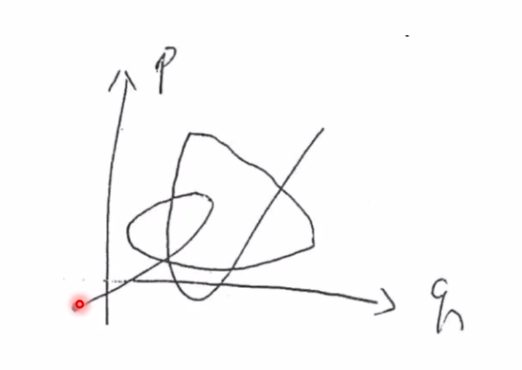
\includegraphics[width=0.5\textwidth]{2-8-phase.png}
	\caption{Example of a Phase Trajectory}
	\label{fig:2-8-phase}
\end{figure}

\subsubsection*{Statistical Ensembles}
A macroscopic system has a very large number of DoF. Tracking details of each DoF at microscopic scale is impractical. Moreover it is impossible to determine exactly the initial value of each degree of freedom.\\

However, we can answer many questions concerning systems in and near thermodynamic equilibrium without knowledge of the motions of individual molecules or atoms.


\subsubsection*{Thermodynamic Equilibrium System}

\begin{example}
	A large isolated system evolving for sufficiently long time.
\end{example}


\end{document}
